\documentclass[12pt,a4paper]{article}
\usepackage[slovene]{babel}
\usepackage[cp1250]{inputenc}
\usepackage[usenames]{color}
\usepackage{pdfpages}
\usepackage{fullpage}
\usepackage{listings}
\begin{document}

\lstset{ %
language=C,                % choose the language of the code
basicstyle=\footnotesize,       % the size of the fonts that are used for the code
numbers=left,                   % where to put the line-numbers
numberstyle=\footnotesize,      % the size of the fonts that are used for the line-numbers
stepnumber=1,                   % the step between two line-numbers. If it's 1 each line will be numbered
numbersep=7pt,                  % how far the line-numbers are from the code
backgroundcolor=\color{white},  % choose the background color. You must add \usepackage{color}
showspaces=false,               % show spaces adding particular underscores
showstringspaces=false,         % underline spaces within strings
showtabs=false,                 % show tabs within strings adding particular underscores
frame=single,	                % adds a frame around the code
tabsize=2,	                % sets default tabsize to 2 spaces
captionpos=b,                   % sets the caption-position to bottom
breaklines=true,                % sets automatic line breaking
breakatwhitespace=false,        % sets if automatic breaks should only happen at whitespace
escapeinside={\%*}{*)}          % if you want to add a comment within your code
}

\begin{titlepage}
\begin{center}
{\Large Univerza v Ljubljani}\\
{\Large Fakulteta za ra�unalni�tvo in informatiko}\\
\vspace{6 cm}
\textbf{{\LARGE Operacijski sistemi 2}}\\
\vspace{2 cm}
\textbf{{\LARGE Kon�no poro�ilo seminarske naloge MAIRM}}\\
\end{center}
\vspace{8.5 cm}

\begin{minipage}{\textwidth}
\begin{flushleft} \large
\textbf{Avtorja:}\\
Matej Jakop, 63070025\newline
Gregor Kali�nik, 63070041
\end{flushleft}
\end{minipage}\\
\vspace{1.0 cm}
\begin{center}
\textbf{Ljubljana, 25. maj 2010}
\end{center}
\end{titlepage}
\setcounter{page}{1}
\tableofcontents
\newpage
\section{Opis izbrane teme in problemskega podro�ja}
Tema seminarske naloge je izdelava virtualne naprave vhodno/izhodnega sistema za popolni nadzor ra�unalnika preko mobilnega telefona pri �emer je povezava med njima vspostavljena preko bluetooth vmesnika. Sama tema seminarske naloge obsega naslednja podro�ja:
\begin{itemize}
\item komunikacij med napravami,
\item poznavanja razli�nih platform (mobilne, ra�unalni�ke),
\item strojnega u�enja (osnove),
\item poznavanje operacijskih sistemov
\end{itemize}
\section{Izbrani cilji, zahteve ter omejitve}
Cilj seminarske naloge je izdelati delujo� sistem in se pri tem nau�iti nove stvari iz podro�ij, ki jih seminarska naloga obsega. Bolj konkretni cilji sistema so:
\begin{itemize}
\item omogo�iti enostavno uporabo sistema,
\item s pomo�jo premikov telefona upravljamo z ra�unalni�ko mi�ko (premiki levo, desno, gor, dol),
\item omogo�iti uporabniku drsenje (scrolling) preko strani s preprostim nagibanjem telefona naprej oziroma nazaj,
\item omogo�iti uporabniku vnos kraj�ih besedil(za dalj�a besedila telefonska tipkovnica ni preve� primerna),
\item omogo�iti uporabniku, da ra�unalnik "nau�i" kako naj bi neka kretnja izgledala,
\item tako "nau�en" ra�unalnik naj bi potem ob uporabnikovi izvedbi kretnje naredil dolo�eno akcijo (npr. zagnal dolo�en program) in
\item vse skupaj narediti z odprtokodnimi orodji/knji�njicami ipd.
\end{itemize}
Ob vseh zgoraj podanih ciljih se pojavi vpra�anja kak�nim zahtevam je potrebno zadostiti, da bo uporaba kon�ne re�itve sploh mo�na. Zahteve za delovanje sistema maj bi bile slede�e:
\begin{itemize}
\item spodoben ra�unalnik z urejeno Java podporo,
\item bluetooth vmesnik,
\item mobilni telefon z merilnikom pospe�ka: v najinem primeru sva se omejila na telefona znamke Nokia s Symbian operacijskim sistemom, kljub temu je prenosljivost na ostale mobilne platforme trivialna.
\end{itemize}
Kot je opaziti iz zahtev re�itev deluje na vseh operacijskih sistemih, kjer je podpora za programski jezik Java. Samo delovanje sistema je bilo testirano na Windows in Linux platformi, kjer je deloval brez te�av.\newline\newline
Po preu�itvi podobnih re�itev na spletu sva pri�la do ugotovitve, da re�itve, ki bi vklju�evala vse najine cilje �e ni na voljo. Obstoje�e re�itve omogo�ajo ve� ali manj samo katero izmed funkcionalnosti/ciljev, ki sva si jih midva zadala. Ena izmed tak�nih re�itev je WiiGee. WiiGee omogo�a u�enje in razpoznavo kretenj. Na �alost/sre�o je ta re�itev osnovana za lastnike igralne konzole Wii. 
\section{Arhitektura re�itve}
\begin{center}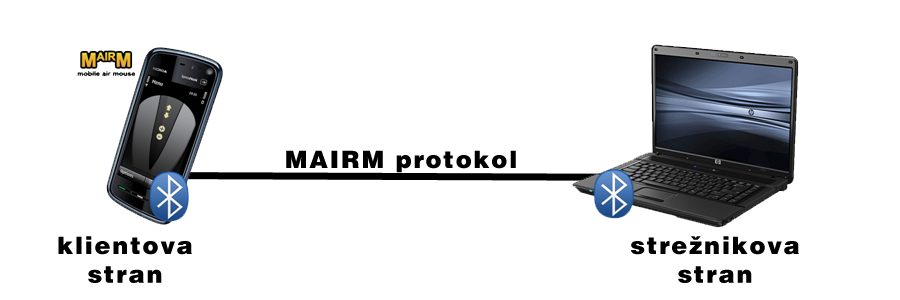
\includegraphics[width=140mm]{images/arch.png}\end{center}
Re�itev je zasnovana s pomo�jo principa stre�nik-odjemalec. Stre�nik in odjemalec med sabo komunicirata preko MAIRM protokola, ki je osnovan na JSON formatu ter je predstavljen v nadaljevanju poro�ila.
\newline\newline
Na stre�nikovi (ra�unalnikovi) strani te�e MAIRM stre�ni�ka aplikacija. Njene naloge so:
\begin{itemize}
\item ustvari bluetooth service (z imenom MAIRM) preko katerega se MAIRM odjemalec pove�e do same aplikacije,
\item poskrbi za pravilno prepoznavo odjemal�evih akcij:
	\begin{itemize}
		\item premikanje mi�ke po zaslonu,
		\item pomikanje po straneh (scrolling),
		\item uporaba mobilne tipkovnice,
		\item prepoznavanje 3D kretenj
	\end{itemize}
\item skrbi za pravilen odziv glede na odjemal�evo akcijo:
	\begin{itemize}
		\item �e zazna zahtevo po premiku mi�ke, premakne mi�ko
		\item �e zazna zahtevo po pomikanje preko strani, simulira potreben dogodek
		\item �e zazna zahtevo po pritisku tipke, simulira pritisk
		\item �e zazna 3D kretnjo naredi akcijo (akcija je dolo�ena v XML datoteki), ki je dolo�ena za njo:
			\begin{itemize}
				\item po�ene nek program
				\item pritisne neko kombinacijo tipk
			\end{itemize}
	\end{itemize}
\end{itemize}
Na mobitelovi strani oziroma odjemal�evi strani te�e MAIRM odjemal�eva aplikacija. Njene naloge so:
\begin{itemize}
\item zajemanje podatkov iz merilnika pospe�ka vgrajenega v sam mobitel,
\item zajemanje pritiskov tipk,
\item posredovanje zajetih podatkov po MAIRM protokolu vse do MAIRM stre�ni�ke aplikacije,
\item skrbi za preklapljanje med naslednjimi na�ini delovanja:
	\begin{itemize}
		\item Mouse mode,
		\item Scrolling mode,
		\item Gesture mode
	\end{itemize}
\item izris uporabni�kega vmesnika za touch screen telefone.
\end{itemize}
Obe komponenti sistema skupaj tvorita delujo�o osnova s katero se (lahko) dose�e zastavljene za�etne cilje.
\subsection{MAIRM protokol}
Sam protol je v JSON formatu in te�e preko Bluetooth Serial Port ter je zelo enostaven. V trenutni verziji je podprta samo enosmerna komunikacija.
\subsubsection{Uporabljeni podatkovni tipi}
boolean  = true ali false\newline
double = decimalno �tevilo\newline
buttonState = up ali down\newline
buttonStateMiddle = up ali down ali scrolling\newline
scrolling pomeni, da telefon preide iz na�ina nadziranja mi�ke na na�in nadziranja scrollerja preko nagibanja\newline
keys = ASCII ali ENTER ali BACKSPACE ali ...\newline
Dodatne tipke so stvar dogovora in potrebe

\subsubsection{Format za GESTURE mode}
Oblika:\newline
\{"gesture":\{"x":"double","y":"double","z":" double ","start":"boolean","end":"boolean"\}\}\newline
Razlaga:\newline
x = vrednost akselometra po x-osi. \newline
Privzeta vrednost: 0.0\newline

y = vrednost akselometra po y-osi.\newline
Privzeta vrednost: 0.0\newline

z = vrednost akselometra po z-osi.\newline
Privzeta vrednost: 0.0\newline

start = dolo�a ali prejeti podatki pomenijo za�etek gesture ali ne. Vrednost true ima lahko samo pri prvem sporo�ilu nekega gesture.\newline
Privzeta vrednost: false\newline\newline
end = dolo�a ali prejeti podatki pomenijo konec gesture ali ne. Vrednost true ima lahko le pri zadnjem sporo�ilu za nek gesture. \newline
Privzeta vrednost: false


\subsubsection{Format za MOUSE mode}
Oblika:\newline
\{"mouse":\{"x":"double","y":"double","z":"double","leftbutton":"buttonState","middlebutton":"buttonStateMiddle","rightbutton":"buttonState"\}\}\newline
Razlaga:\newline
x = vrednost akselometra po x-osi. \newline
Privzeta vrednost: 0.0\newline

y = vrednost akselometra po y-osi.\newline
Privzeta vrednost: 0.0\newline

z = vrednost akselometra po z-osi.\newline
Privzeta vrednost: 0.0\newline
leftbutton = levi mi�kin gumb\newline
Privzeta vrednost: up\newline
middlebutton = srednji mi�kin gumb\newline
Privzeta vrednost: up\newline
rightbutton = desni mi�kin gumb\newline
Privzeta vrednost: up\newline

\subsubsection{Format za KEYBOARD mode}
Oblika:\newline
\{"keyboard": \{"key":"keys"\}\}\newline
Razlaga:\newline
key = tipka, ki naj bi bila pritisnjena na ra�unalni�ki tipkovnici


\section{Izvedba re�itve in problemi pri tem}
Sama izvedba re�itve na prvi pogled izgleda �isto enostavna. Ko pa se zatopimo v delo in posku�amo re�itev dejansko izvesti, pa pridemo do razli�nih problemov, ki jih je potrebno re�iti. Midva sva pri�la do naslednjih problemov:
\begin{enumerate}
\item Vzpostavitev povezave med razli�nimi napravami
\item Pridobitev podatkov iz pospe�kometra v mobilnem telefonu
\item Simulacija delovanja mi�ke in tipkovnice
\item U�enje in razpoznava kretenj
\end{enumerate}
Vse na�tete probleme, ki so bolj podrobno opisani v nadaljevanju, sva uspe�no re�ila.

\subsection{Pregled uporabni�kega vmesnika}
Uporabni�ki vmesnik kot tak se nama ni zdel bistven del zato mu nisva posve�ala preve� pozornosti. Bolj sva se osredoto�ila na samo ozadje re�itve.
\subsubsection{Osnovno okno}
\textbf{Osnovno okno, ki ga odbimo ob zagonu:}
\begin{center}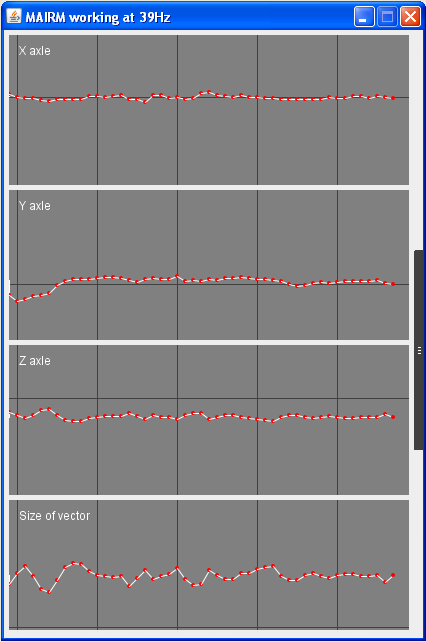
\includegraphics[width=140mm]{images/ui_main.png}\end{center}
\textbf{Raz�irjeno okno za vnos/u�enje kretnje:} Ra�irjeno okno dobimo po kliku na temno sivi zavihek.
\begin{center}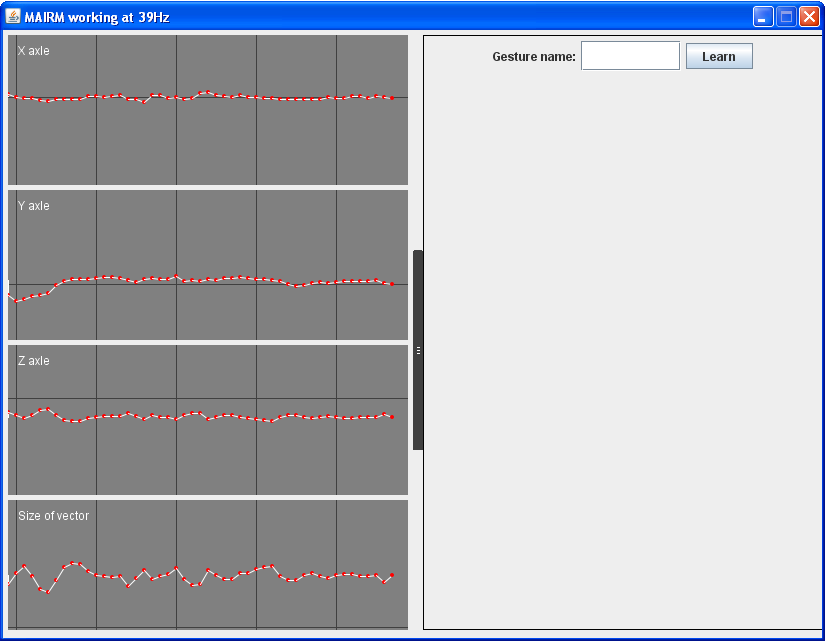
\includegraphics[width=140mm]{images/ui_main_ext.png}\end{center}
\subsubsection{Delovanje v ozadju}
Po minimizaciji glavnega okno gre sistem v delovanje v ozadju. Ko je sistem v tem na�inu delovanja se na mestu poleg ure pojavi ikonca, ki predstavlja program.
\begin{center}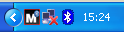
\includegraphics[width=40mm]{images/ui_main_back.png}\end{center}
Ko se v sistem pove�e telefon ikonca spremeni svojo barvo in s tem je ponazorjena uspe�na povezava.
\begin{center}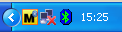
\includegraphics[width=40mm]{images/ui_main_back_connected.png}\end{center}
\subsubsection{Uporabni�ki vmesnik na mobilnem telefonu}
Uporabni�ki vmesnik na mobilnem telefonu ni ni� posebnega, saj po tem ni potrebe. Potrebno bistvo se skriva v ozadju.
\subsection{Vzpostavitev povezave med razli�nimi napravami}
\subsubsection{Opis problema:}
Imamo dve napravi, ki sta obe sposobni bluetooth komunikacije. Pri tem se pojavijo naslednja vpra�anja:
\begin{enumerate}
\item Katera izmed naprav naj bo gospodar, ki prejema zahteve po povezavi od druge naprave?
\item Kako programsko, hitro in �imbolj enostavno vzpostaviti povezavo s pogojem, da to deluje na vseh sistemih?
\end{enumerate}

\subsubsection{Opis re�itve:}

\begin{enumerate}
\item Ta problem sva re�ila zelo enostavno. Ker je potrebno za delovanje sistema oziroma samo sporo�anje premikov telefona zagnati aplikacijo na mobilniku (predpostavljava, da je na ra�unalniku �e pognana), sva se odlo�ila, da naj bo mobilnik tisti, ki poda zahtevo po vzpostavitvi povezave. Tako je tudi re�eno, da ni potrebno aplikaciji na ra�unalniku skenirati na okoli za napravami, ki imajo MAIRM sposobnost. S tem se prihrani nekaj tudi na energijski porabi (ki je sploh na prenosnih napravah klju�nega pomena), ker se povezava vzpostavlja in ostaja aktivna samo takrat, ko je dejansko potrebna.
\item Naslednji problem je �e bil malce te�ji. Te�ji iz vidika, da �eliva to po�eti preko programskega jezika Java in to na vseh platformah. Po brskanju na spletu sva pri�la do knji�njice BlueCove, ki omogo�a to�no to kar potrebujeva. Potem je bilo potrebno samo �e spoznati uporabo te knji�njice in standard, ki je osnova implementacije. Kon�na implemetacija povezave je bila re�ene na slede�i na�in: 
	\begin{enumerate}
		\item Stre�ni�ka aplikacija na ra�unalniku ob zagonu kreira storitev z imenom MAIRM. Storitev te�e na vrhu protokola Bluetooth Serial Port Profile,
		\item Uporabnik po zagonu MAIRM mobilne aplikacije dobi na voljo izbiro bluetooth naprave ter nato �e izbiro storitve (v primeru, da bi bilo storitev ve� ali pod razli�nimi imeni)
		\item �e je vse pravilno storjeno, se komunikacija vzpostavi.
	\end{enumerate}
	\end{enumerate}

\subsection{Pridobitev podatkov iz pospe�kometra v mobilnem telefonu}
\subsubsection{Opis problema:}
�e od samega za�etka sva vedela katere mobilne telefone bova uporabila pri najini seminarski nalogi. Preostala je le �e izbira programskega jezika v katerem se je mogo�e dokopati do teh podatkov in kako to storiti v izbranem programskem jeziku.
\subsubsection{Opis re�itve:}
Za programiranje na Symbian platformi imamo na voljo naslednje programske jezike:
\begin{itemize}
	\item Java
	\item C/C++
	\item Python
\end{itemize}
Od vseh mo�nosti najprej odpade programski jezik Java, ker nima (�e) dodanega aplikacijskega vmesnika do senzorjev, ki so v telefonu. Zaradi enostavnosti implementacije sva izbrala programski jezik Python, �eprav se v samem interpreterju jezika in dokumentaciji pojavljajo napake. Osnovna implementacija v Pythonu je naslednja: 
\begin{enumerate}
	\item uporabi razred sensor in mu podaj funkcijo/metodo za katero �eli�, da se kli�e ob dogodkih vzor�enja podatkov iz senzorja
	\item v klicani metodi po�lji podatke na ra�unalnik
\end{enumerate}
Ob tem velja omeniti, da je potrebno re�iti izgubljanje podatkov v primeru napake pri po�iljanju podatkov preko bluetooth vmesnika.

\subsection{Simulacija delovanja mi�ke in tipkovnice}
\subsubsection{Opis problema:} Pri seminarski nalogi sva pri�la do to�ke, ko je bilo potrebno za�eti simulirati delovanje mi�ke in tipkovnice. Torej, �elela sva programsko operacijskemu sistemu sporo�iti, da se je mi�ka premaknila desno, da se je zgodil klik,....
\subsubsection{Re�itev problema:} Sprva sva mislila, da bo v Javi to problem, ki ga bo potrebno re�evati preko JNI (java native interface). Kar bi celotno implementacijo malce ote�ilo. Na sre�o sva pri�la do spoznanja, da obstaja razred Robot, ki omogo�a vse kar sva potrebovala. Z razredom Robot je mogo�e:
\begin{itemize}
	\item Zajemati zaslonsko sliko,
	\item Premikati mi�ko,
	\item Pritiskati tipke,
	\item Izvajati drsenje po straneh(scrollanje)
	\item ...
\end{itemize}
Dobra stvar tega razreda je tudi ta, da je �e vsebovan v standardni Javi.

\subsection{U�enje in razpoznava kretenj}
\subsubsection{Opis problema:} Iz prejetih podatkov, ki jih dobiva iz mobilnega telefona je bilo potrebno nekako zagotoviti, da bo sistem znal prepoznati, kaj je uporabnik izvedel. Npr. uporabnik v zraku nari�e krog in sistem ga uspe�no prepozna. Sprva se nama je problem zdel te�ek in ob enem zanimiv, kar je samo dal dodatno motivacijo za njegovo razre�itev.
 
\subsubsection{Re�itev problema:}
Problem sva �elela re�iti na ve� bolj ali manj uspe�nih postopkov:
\begin{enumerate}
	\item \textbf{Poskus odkrivanje v katero izmed smeri se gibje telefon (gor, dol, levo, desno, postrani v levo...):} Delovanje sistema na tak na�in bi bilo bolj slabo, �eprav je v teoriji vsaj v enem delu izgledal obetavno (ne bi pri�lo do napa�nih detekcij, detekcija bi bila ali pa ne). Problem bi bil v tem, da bi te�ko prepoznaval krivulje ter, da bi bilo pri izvajanju potrebno zagotoviti ostre prehode med posameznimi smermi (uporabnik bi moral delat zelo nazorne gibe).
	\item \textbf{Uporaba algoritma strojnega u�enja k-nearest neighbours:} Idejo za ta algoritem sva dobila po pregledu diplomske naloge �tudenta iz na�e fakultete. Dodatno motivacijo za uporabo slede�ega algoritma sva dobila �e zaradi zelo dobrih rezultatov prepoznavanja, ki jih je dosegel pri svojem delu. 
\end{enumerate}

Torej za re�itev problema u�enja in razpoznave kretenj sva izbrala algoritem strojnega u�enja k-nearest neighbours. Edina slabost te izbire je, da algoritem ni med najhitrej�imi pri sami razpoznavi. Vzrok tega je, da se sistem ne u�i ampak �ele pri razpoznavi posku�a klasificirati kateremu razredu (kretnji) pripada nek seznam vrednosti. Kljub temu, se nama je zdel dobra nalo�ba. Sam algoritem pri svojem delovanju uporablja ra�unanje razdalje med dvema zaporedjema. Ker se vrednosti pri izvajanju kretnje lahko �asovno razlikujejo (nek gib ne izvedemo vedno �asovno �isto enako) sva za merjenje razdalje uporabila algoritem DTW (dynamic time warp). Osnovna implementacija obeh algoritmov je dokaj enostavna, a po�asna. �e bi �elela hitro implementacijo bi bilo potrebno precej ve� dela za dosego spodnje meje implementacije. Zato sva raje uporabila �e obstoje�o re�itev s tega podro�ja, in sicer implementacijo v java programski knji�njici JML (java machine learning). Po preu�itvi uporabe knji�njice je bil problem re�en.


\section{Morebitno nadaljnje delo}
Projekt je objavljen na google code (http://code.google.con/p/mairm/) in kot tak je na voljo vsem, ki bi radi kaj dodali/spremenili. Torej odprte so vse opcije za sodelovanje drugih ljudi in tem uresni�evanje njihovih idej. Kot uporabnika in razvijalca sistema sva pri�la do ugotovitve, da bi bilo dobro za bolj�o uporabni�ko izku�njo narediti �e slede�e stvari:
\begin{enumerate}
\item V XML datoteko uvesti pogoje glede na trenutno aktivno aplikacijo. Tako bi se lahko zagotovilo, da bi ista kretnja imela razli�en pomen v razli�nih programih. Npr. kretnja v desno bi v predvajalniku glasbe prestavila na drugo pesem, medtem ko v pregledovalniku slik na naslednjo sliko.
\item Nekako poskrbeti, da bi sistem sam izbolj�eval svoje znanje o kretnjah (brez sodelovanja uporabnika pri temu).
\item Prestaviti delovanje programa na vi�ji prioritetni nivo (ker se druga�e zna zgoditi, da ob veliki zasedenosti ra�unalnika celoten sistem deluje upo�asnjeno in ne tako kot prava mi�ka), �eprav je ta pojav redek.
\end{enumerate}
Bistveno za nadaljnje delo je to, da morava poskrbeti, da bo ve� ljudi spoznalo najin projekt in ga morebiti za�elo uporabljati. Le-tako bo smiselno dodajati nove funkcionalnosti in izbolj�ave. �e neka re�itev nima uporabnikov, vsak (pa naj bo �e tako dober) projekt slej ko prej umre. Kar je v�asih �koda.

\section{Navodila za uporabo}
\subsection{Zahteve za delovanje sistema}
Zahteve za delovanja sistema so skromne. Potrebno je imeti le:
\begin{itemize}
\item Operacijski sistem Windows/Linux/Mac
\item ra�unalnik z bluetooth vmesnikom
\item mobilni telefon znamke Nokia s Symbian S60 3rd Edition ali Nokia s Symbian S60 5rd Edition, name��eno python podporo (pyS60) in prisotnost merilnika pospe�ka v samem telefonu
\end{itemize}
Zadnja to�ka seznama se bo lahko s �asom malce posplo�ila. V prihodnosti projekta bo verjetno dovolj, da bo uporaben poljuben telefon z merilnikom pospe�ka.

\subsection{Potek namestitve}
\subsubsection{Mobilni telefon}
Mo�nih je ve� opcij:
\begin{enumerate}
\item V primeru �e name��enega pyS60 na mobilni telefon prenesemo (preko bluetooth ali kako druga�e) samo mairm.py datoteko, ki se nahaja v paketu za in�talacijo. Na mobilnem telefonu jo shranimo na pomnilni�ko kartico v imenik data/python. Tako bo datoteka vidna v python vmesniku do interpreterja. Namestitev kon�ana.
\item V primeru, da je v namestitvenemu paketu prisotna datoteka mairm.sis le-to prenesemo na mobilni telefon in po�enemo namestitev ter sledimo korakom na zaslonu.
\end{enumerate}

\subsubsection{Ra�unalnik}
Na ra�unalniku je namestitev sila preprosta. Potrebno je samo razpakirati namestitveni paket ali pognati namestitveno datoteko.

\subsection{Povezava mobilnega telefona in ra�unalnika ter pri�etek delovanja}
Za vzpostavitev povezave je potrebno slediti naslednjim korakom:
\begin{enumerate}
\item Vklopimo bluetooth vmesnik v kolikor je izklju�en
\item Sparimo telefon in ra�unalnik v primeru, daj eto potrebno storiti
\item Po�enemo program MAIRM (�e smo namestili z namestitvenim programom) oziroma v direktoriju namestitvenega pakete v konzoli po�enemo ukaz 
\begin{center}
java -jar mairm.jar
\end{center}
\item Na mobilnem telefonu po�enemo aplikacijo MAIRM (�e smo namestili z mairm.sis ) oziroma Python 2.x.x. �e smo pognali Python 2.x.x moramo v njem �e odpreti skripto. To storimo tako, da izberemo \"options\" in nato \"run script\". Poi��emo datoteko mairm.py in jo izberemo. 
\item Prika�e se nam seznam bluetooth naprav in izberemo na� ra�unalnik na katerem te�e mairm. Po potrditvi tega nas bo telefon morebiti �e povpra�al po storitvi na katero se �elimo povezati. Enostavno izberemo MAIRM.
\item �e so bili vsi koraki uspe�no izvedeni, bi se sedaj morala mi�ka za�eti premikati po zaslonu v skladu s premikanjem telefona.
\end{enumerate}


\subsection{Uporabni napotki pri uporabi}
\subsubsection{Mi�ko premikamo ekranu v skladu s temi na�eli:}
\begin{itemize}
\item Nagib telefona naprej, premakne mi�ko navzgor,
\item Nagib telefona nazaj, premakne mi�ko navzdol,
\item Nagib telefona levo, premakne mi�ko levo,
\item Nagib telefona desno, premakne mi�ko desno,
\item Pritisk leve akcijske tipke na telefonu povzro�i levi klik,
\item Pritisk desne akcijske tipke na telefonu povzro�i desni klik
\item Pritisk na tipko za izbiro na telefonu povzro�i:
	\begin{itemize}
		\item Preklop na na�in drsenja (scrolling mode) ali
		\item Za�etek zajemanja izvajanja kretnje
	\end{itemize}
	Katera stvar se bo zgodila je odvisno od tega, koliko �asa dr�imo tipko. �e jo dr�imo dlje kot 100ms potem za�ne izvajati na�in kretnje (gesture mode), druga�e pa enostavno anredi preklop.
\item Pritisk tipke urejanje (edit, svin�nik) povzro�i, da se pojavi okno v katerega vnesemo besedilo, ki se naj izpi�e na ra�unalniku.
\end{itemize}

\subsubsection{Novo kretnjo posnamemo na slede�i na�in:}
\begin{enumerate}
\item Odpremo glavno okno aplikacije (�e se aplikacija slu�ajno skriva v System tray podro�ju)
\item Aplikacijo raz�irimo s klikom na sivi gumb, da dobimo opcijo vnosa imena kretnje
\item Vnesemo ime kretnje ter kliknemo na Learn
\item S pomo�jo telefona (seveda mora biti najprej vzpostavljena povezava med mobitelom in ra�unalnikom) izvedemo kretnjo kot obi�ajno
\item �e �e nismo tega storili vsaj 5x se vrnemo 3. korak in ponovimo z istim imenom
\item �e �e nimamo shranjeni vsaj 2 kretnji, ponovimo postopek vendar tokrat z drugo kretnjo.
\item Ko vse opravimo kot je bilo opisano v prej�njih korakih, bi moral sistem za�eti prepoznavati uporabnikove definirane kretnje
\end{enumerate}

\subsubsection{Nastavitev kaj naj sistem naredi ob izvedbi dolo�ene kretnje}
\begin{enumerate}
\item Odpremo datoteko actions.xml, ki se nahaja v istem direktoriju, kot je bil name��en sam program.
\item V datoteki bi �e moral biti prisoten seznam vseh kretenj, ki jih sistem pozna. 
\item Odlo�iti se je potrebno kaj bi radi, da sistem naredi:
	\begin{itemize}
		\item izvede nek program\newline
			V tem primeru med zna�ke $<$exec$>$ in $<$/exec$>$ vnesemo pot in ime programa.
		\item pritisne dolo�eno kombinacijo tipk\newline
			V tem primeru med zna�ke $<$keys$>$ in $<$/keys$>$ dodamo nove tipke in sicer podobno kot v em primeru:
			\begin{center} $<$key delayRelease="false"$>$F1$<$/key$>$ \end{center}
			To pomeni, da se bo v primeru izvedbe kretnje simuliral pritisk tipke F1. Atribut delayRelease pa pomeni ali naj sistem dr�i tipko vse dokler se ne izvedejo �e preostali pritiski tipk. �e en primer tega za po�iljanje windows+r (po�ene okno za zagon programa):
			\begin{center} $<$key delayRelease="true"$>$WINDOWS$<$/key$>$\end{center}
			\begin{center} $<$key delayRelease="false"$>$r$<$/key$>$ \end{center}
			Seznam vseh tipk, ki so na voljo za tak�en vnos je zapisan v datoteki keyboard\_keys\_available.txt po prvem zagonu MAIRM programa.
	\end{itemize}
\item Datoteko shranimo
\item Kliknemo z desno mi�kino tipko na ikonco mairm programa in izberemo opcijo \"Reload gesture action bindings\".
\end{enumerate}

\subsubsection{Izbolj�ava zaznavanja kretenj}
�e se opazi, da sistem dve kretnji pogosto zamenjuje potem lahko to re�ite dokaj enostavno. Potrebno je posneti samo ve� ponovitev problemati�nih kretenj (pri �tevilu 15x ponovitev sistem �e zelo dobro lo�i tudi skoraj �isto enake kretnje, npr. krog v levo in krog v desno). 












\newpage
\addcontentsline{toc}{section}{Literatura} 
\begin{thebibliography}{1}
\bibitem{kononenko}
Kononenko, I. (1997). Strojno u�enje. Ljubljana: Fakulteta za ra�unalni�tvo in informatiko.
\bibitem{bluecove}
BlueCove documentation.[Online].[Citirano: 2. april 2010; 18:00]. Dostopno na spletnem naslovu: http://code.google.com/p/bluecove/wiki/Documentation
\bibitem{jml}
Java machine learning.[Online].[Citirano: 2. april 2010; 19:00]. Dostopno na spletnem naslovu: http://java-ml.sourceforge.net/content/getting-started
\bibitem{diploma}
Strle, B. (2008). Prepoznavanje �love�kih gibov s pospe�kometri in strojnim u�enjem. Ljubljana: Fakulteta za ra�unalni�tvo in informatiko.
\end{thebibliography}
\end{document}